% Source: graduate-coursework/Research/Intro_to_Agents/handouts/Part8_Advanced_Topics.tex

\documentclass[border=4pt]{standalone}
\usepackage[T1]{fontenc}
\usepackage{graphicx}
\usepackage{lmodern}
\usepackage{tikz}
\usepackage{xcolor}
\usetikzlibrary{shapes.geometric, arrows.meta, positioning, calc, fit, backgrounds, matrix, decorations.pathreplacing}

\definecolor{UofSCGarnet}{HTML}{73000a}
\definecolor{UofSCBlack}{HTML}{000000}
\definecolor{UofSCWhite}{HTML}{ffffff}
\definecolor{UofSCRose}{HTML}{CC2E40}
\definecolor{UofSCAtlantic}{HTML}{466A9F}
\definecolor{UofSCCongaree}{HTML}{1F414D}
\definecolor{UofSCHorseshoe}{HTML}{65780B}
\definecolor{UofSCGrass}{HTML}{CED318}
\definecolor{UofSCHoneycomb}{HTML}{A49137}
\definecolor{UofSC90Black}{HTML}{363636}
\definecolor{UofSC70Black}{HTML}{5C5C5C}
\definecolor{UofSC50Black}{HTML}{A2A2A2}
\definecolor{UofSCWarmGrey}{HTML}{676156}
\definecolor{UofSCSandstorm}{HTML}{FFF2E3}
\definecolor{UofSCDarkGarnet}{HTML}{570008}
\definecolor{UofSCAzalea}{HTML}{844247}

\tikzset{
    % Sharp corners for all nodes
    every node/.style={font=\small},
    % Process box style
    process/.style={
        rectangle,
        draw=UofSCBlack,
        fill=UofSCWhite,
        minimum width=2.5cm,
        minimum height=0.8cm,
        align=center,
        font=\footnotesize
    },
    % Decision box style
    decision/.style={
        diamond,
        draw=UofSCBlack,
        fill=UofSCSandstorm,
        minimum width=2cm,
        minimum height=1cm,
        align=center,
        font=\footnotesize,
        aspect=2
    },
    % Start/End style
    startstop/.style={
        rectangle,
        draw=UofSCGarnet,
        fill=UofSCGarnet,
        text=UofSCWhite,
        minimum width=2cm,
        minimum height=0.7cm,
        align=center,
        font=\footnotesize\bfseries
    },
    % Arrow style
    arrow/.style={
        ->,
        >=Stealth,
        thick,
        color=UofSCBlack
    },
    % Failure node
    failure/.style={
        rectangle,
        draw=UofSCRose,
        fill=UofSCRose!20,
        minimum width=2cm,
        minimum height=0.7cm,
        align=center,
        font=\footnotesize
    },
    % Success node
    success/.style={
        rectangle,
        draw=UofSCHorseshoe,
        fill=UofSCHorseshoe!20,
        minimum width=2cm,
        minimum height=0.7cm,
        align=center,
        font=\footnotesize
    },
    % Highlight box
    highlight/.style={
        rectangle,
        draw=UofSCGarnet,
        fill=UofSCGarnet!10,
        line width=1.5pt,
        minimum width=2.5cm,
        minimum height=0.8cm,
        align=center,
        font=\footnotesize
    },
    % Security threat style
    threat/.style={
        rectangle,
        draw=UofSCRose,
        fill=UofSCRose!15,
        minimum width=2.2cm,
        minimum height=0.7cm,
        align=center,
        font=\footnotesize
    },
    % Agent node
    agent/.style={
        rectangle,
        draw=UofSCAtlantic,
        fill=UofSCAtlantic!15,
        minimum width=2.2cm,
        minimum height=0.8cm,
        align=center,
        font=\footnotesize
    },
    % Human node
    human/.style={
        rectangle,
        draw=UofSCCongaree,
        fill=UofSCCongaree!15,
        minimum width=2.2cm,
        minimum height=0.8cm,
        align=center,
        font=\footnotesize
    },
    % Cost node
    cost/.style={
        rectangle,
        draw=UofSCHoneycomb,
        fill=UofSCHoneycomb!20,
        minimum width=2cm,
        minimum height=0.7cm,
        align=center,
        font=\footnotesize
    },
    % Test node
    test/.style={
        rectangle,
        draw=UofSCAtlantic,
        fill=UofSCAtlantic!10,
        minimum width=2cm,
        minimum height=0.7cm,
        align=center,
        font=\footnotesize
    },
    % Pipeline stage
    pipeline/.style={
        rectangle,
        draw=UofSCCongaree,
        fill=UofSCCongaree!10,
        minimum width=2.5cm,
        minimum height=0.8cm,
        align=center,
        font=\footnotesize
    },
    % Timeline event
    timeline/.style={
        rectangle,
        draw=UofSCGarnet,
        fill=UofSCWhite,
        minimum width=1.8cm,
        minimum height=0.6cm,
        align=center,
        font=\tiny
    }
}

\begin{document}
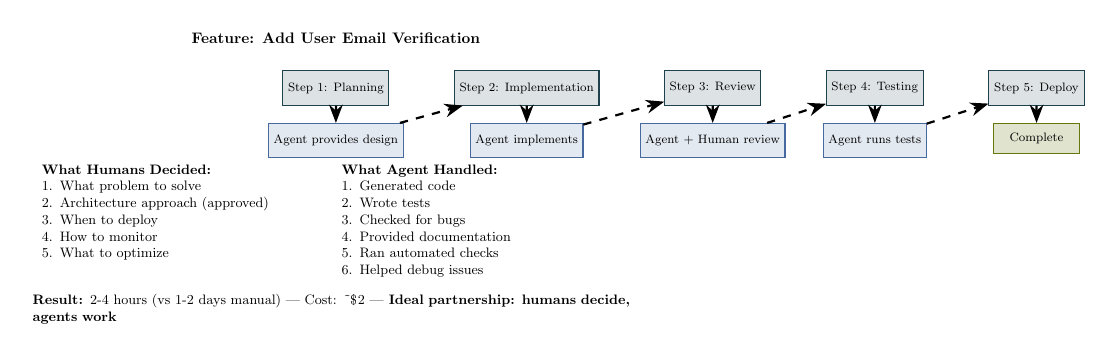
\begin{tikzpicture}[node distance=0.4cm and 0.8cm, scale=0.55, transform shape]
        % Timeline
        \node (title) [font=\bfseries] {Feature: Add User Email Verification};

        \node (step1) [human, below=0.5cm of title] {Step 1: Planning};
        \node (a1) [agent, below=of step1] {Agent provides design};

        \node (step2) [human, right=1.5cm of step1] {Step 2: Implementation};
        \node (a2) [agent, below=of step2] {Agent implements};

        \node (step3) [human, right=1.5cm of step2] {Step 3: Review};
        \node (a3) [agent, below=of step3] {Agent + Human review};

        \node (step4) [human, right=1.5cm of step3] {Step 4: Testing};
        \node (a4) [agent, below=of step4] {Agent runs tests};

        \node (step5) [human, right=1.5cm of step4] {Step 5: Deploy};
        \node (a5) [success, below=of step5] {Complete};

        \draw [arrow] (step1) -- (a1);
        \draw [arrow] (step2) -- (a2);
        \draw [arrow] (step3) -- (a3);
        \draw [arrow] (step4) -- (a4);
        \draw [arrow] (step5) -- (a5);

        \draw [arrow, dashed] (a1) -- (step2);
        \draw [arrow, dashed] (a2) -- (step3);
        \draw [arrow, dashed] (a3) -- (step4);
        \draw [arrow, dashed] (a4) -- (step5);

        % Details below
        \node [below=2.5cm of title, text width=14cm, font=\small] {
            \begin{tabular}{p{6.5cm}p{6.5cm}}
                \textbf{What Humans Decided:} & \textbf{What Agent Handled:}\\
                1. What problem to solve & 1. Generated code\\
                2. Architecture approach (approved) & 2. Wrote tests\\
                3. When to deploy & 3. Checked for bugs\\
                4. How to monitor & 4. Provided documentation\\
                5. What to optimize & 5. Ran automated checks\\
                & 6. Helped debug issues\\
            \end{tabular}

            \vspace{0.3cm}
            \textbf{Result:} 2-4 hours (vs 1-2 days manual) | Cost: \textasciitilde\$2 | \textbf{Ideal partnership: humans decide, agents work}
        };
    \end{tikzpicture}
\end{document}
